\section{Threshold and search of contours}
To measure a object bypassing the camera field the outlines of the object are needed. The challenge here is to find the edges of an object with little computing power in such a short time that the measurement time does not become useless. For further processing the edges have to be represented by an one pixel thick line. This section shows the used method and implementation of the further used edge detection. The ISP driver of the Jetson Nano is used in the automatic mode. In this configuration the ISP tries to keep the mean of the image close to the value 128, which resembles the middle of its range. Since the gStreamer pipeline handling over Python is somewhat complicated, the camera is only used in automatic mode.

\subsection{Threshold}
To determine a good threshold method a short look at the histogram is the first step to success. With a back light it can be expected to have a clear difference between foreground and background of the image. 
\begin{figure}[ht]
	\subfigure[\label{development:thre1}]{\fbox{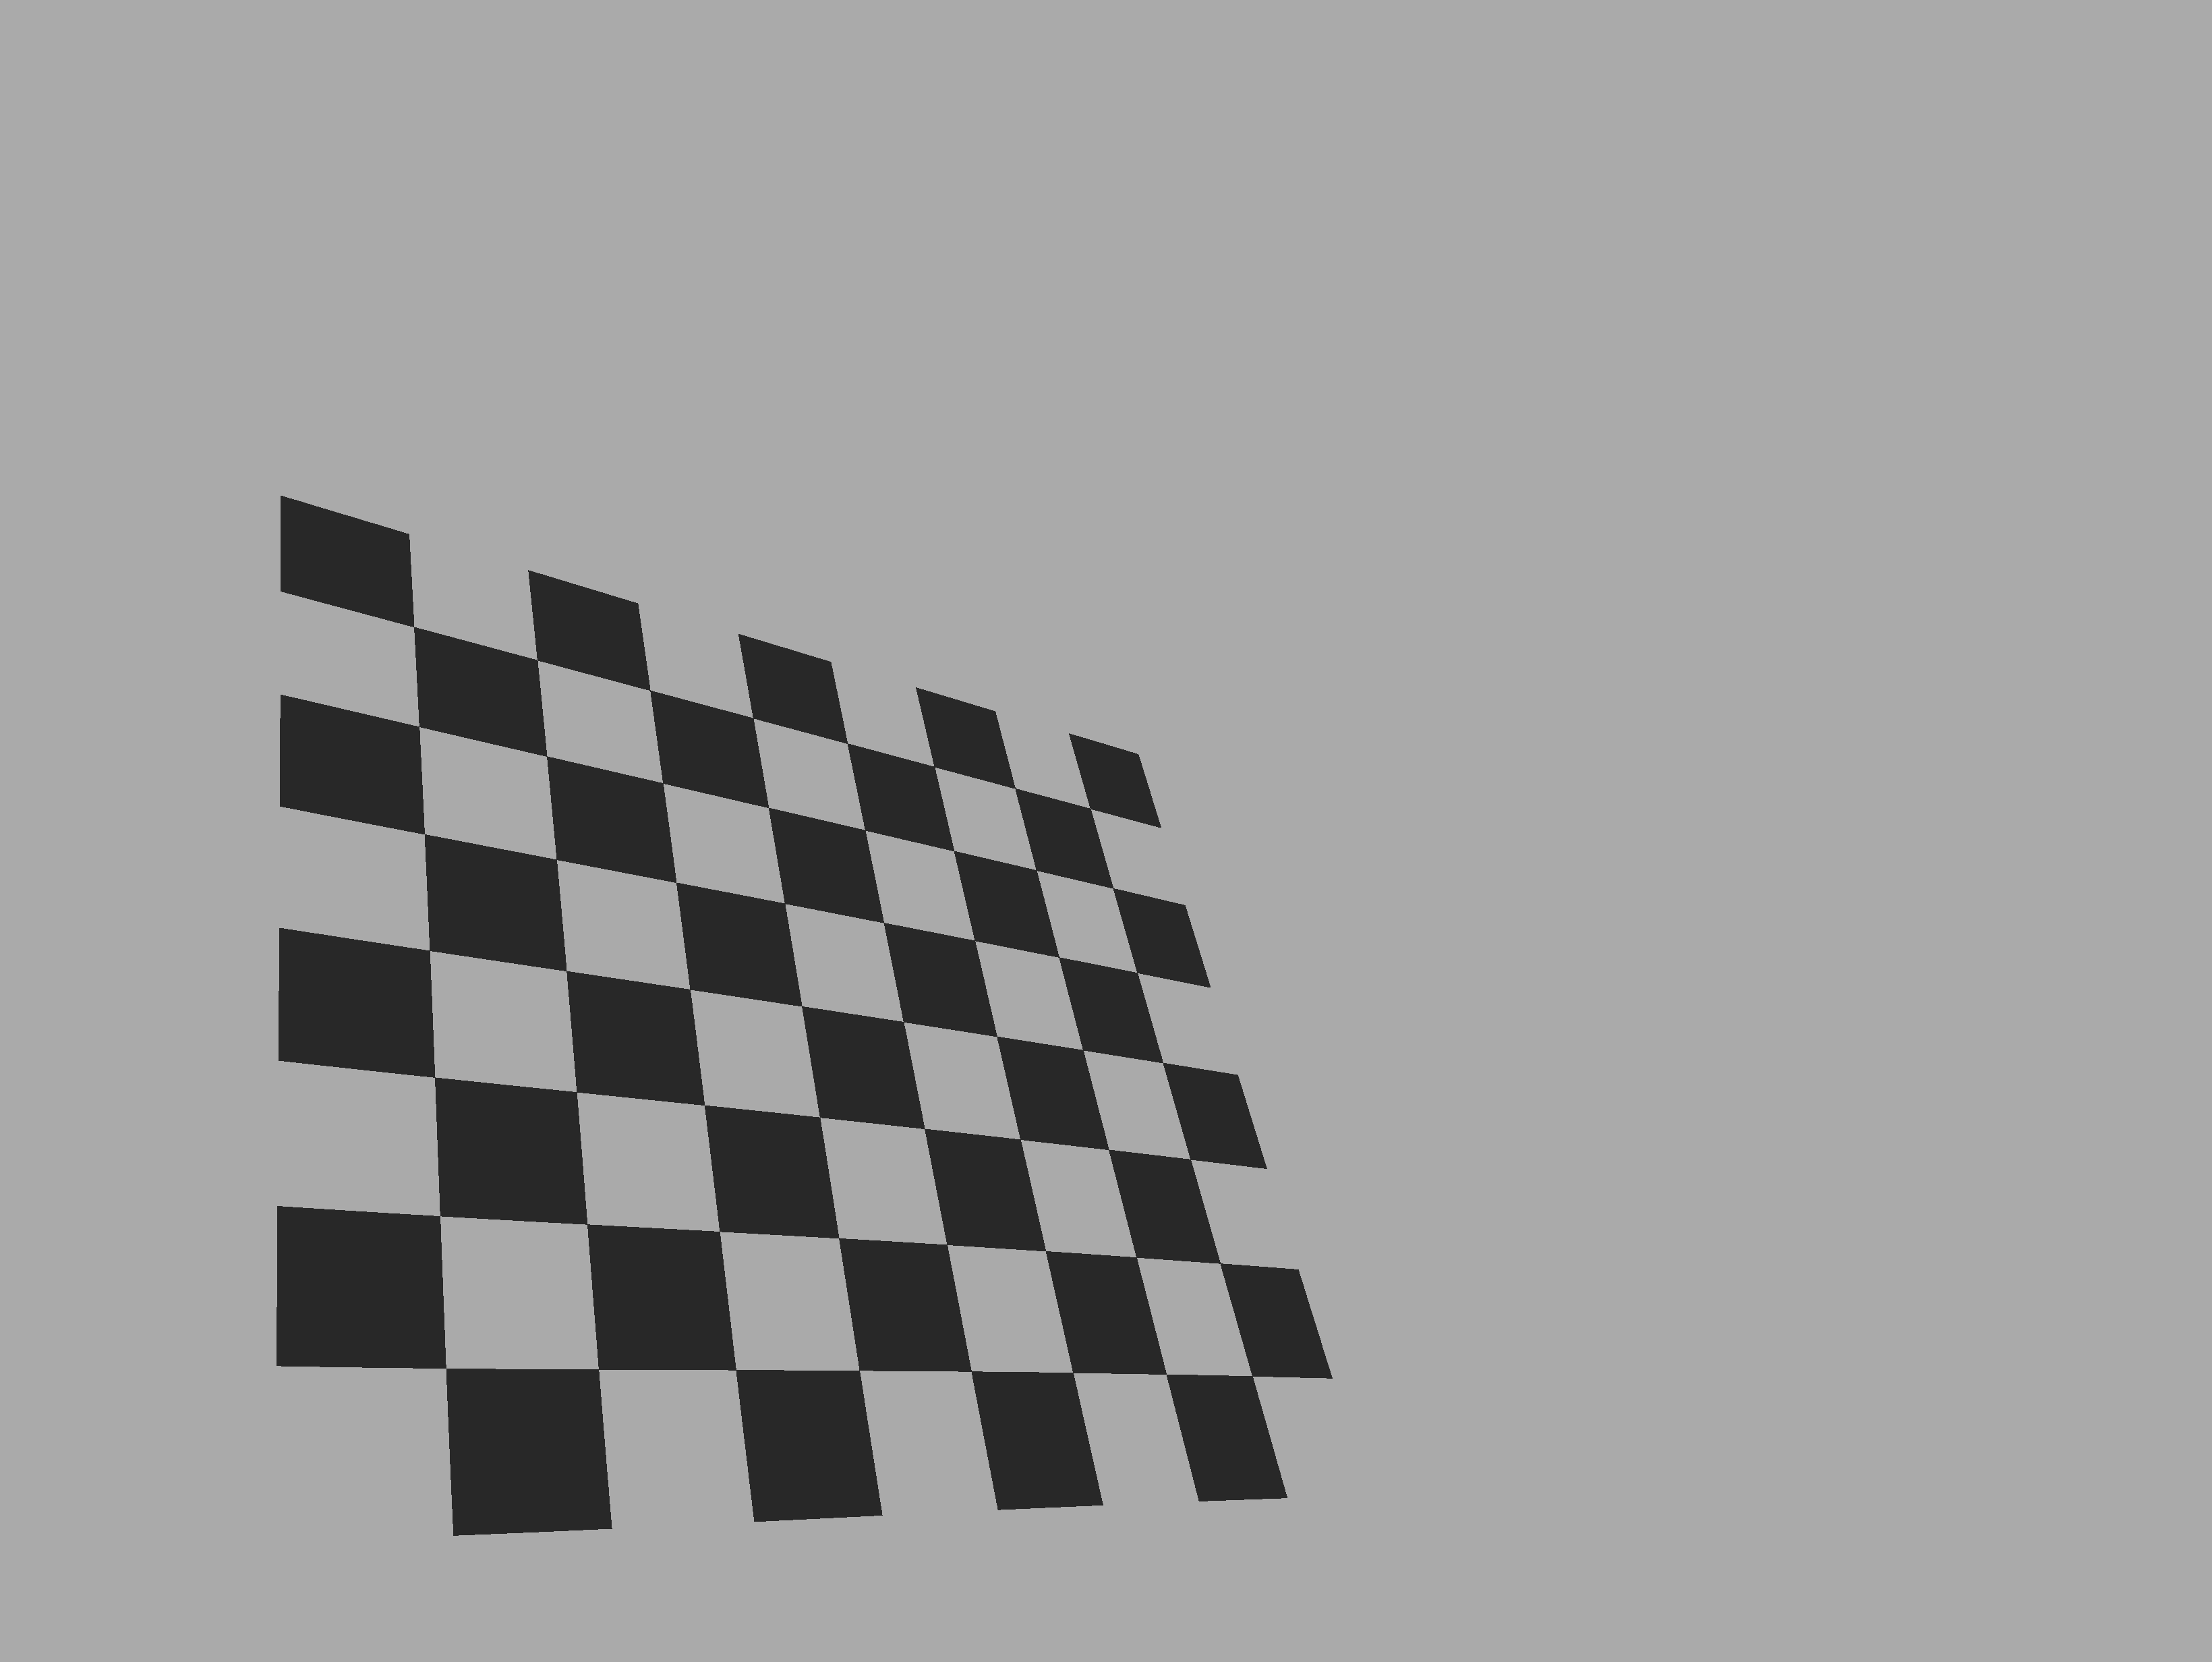
\includegraphics[width=0.5\linewidth, height=5cm]{3-development/threshold/im0.png}}}
	\subfigure[\label{development:thre2}]{\fbox{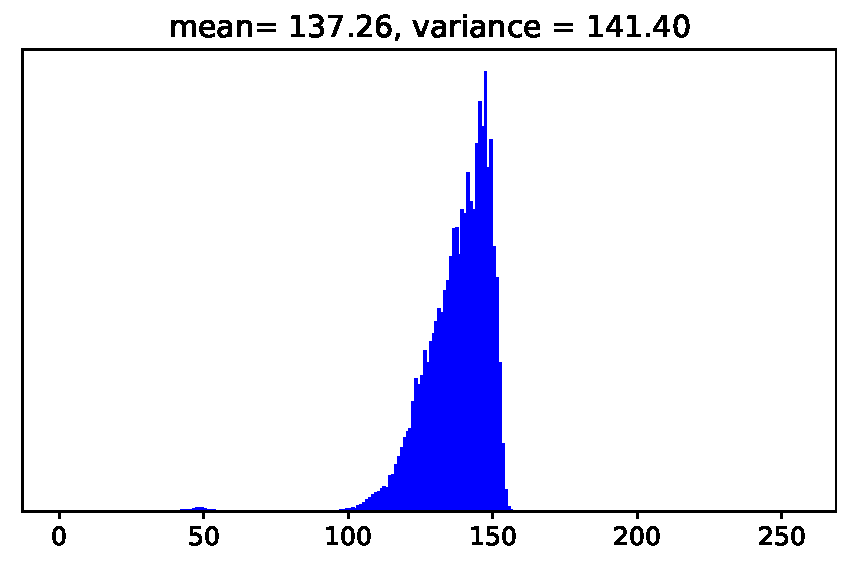
\includegraphics[width=0.5\linewidth, height=5cm]{3-development/threshold/hist_pattern2.pdf}}}
	\subfigure[\label{development:thre3}]{\fbox{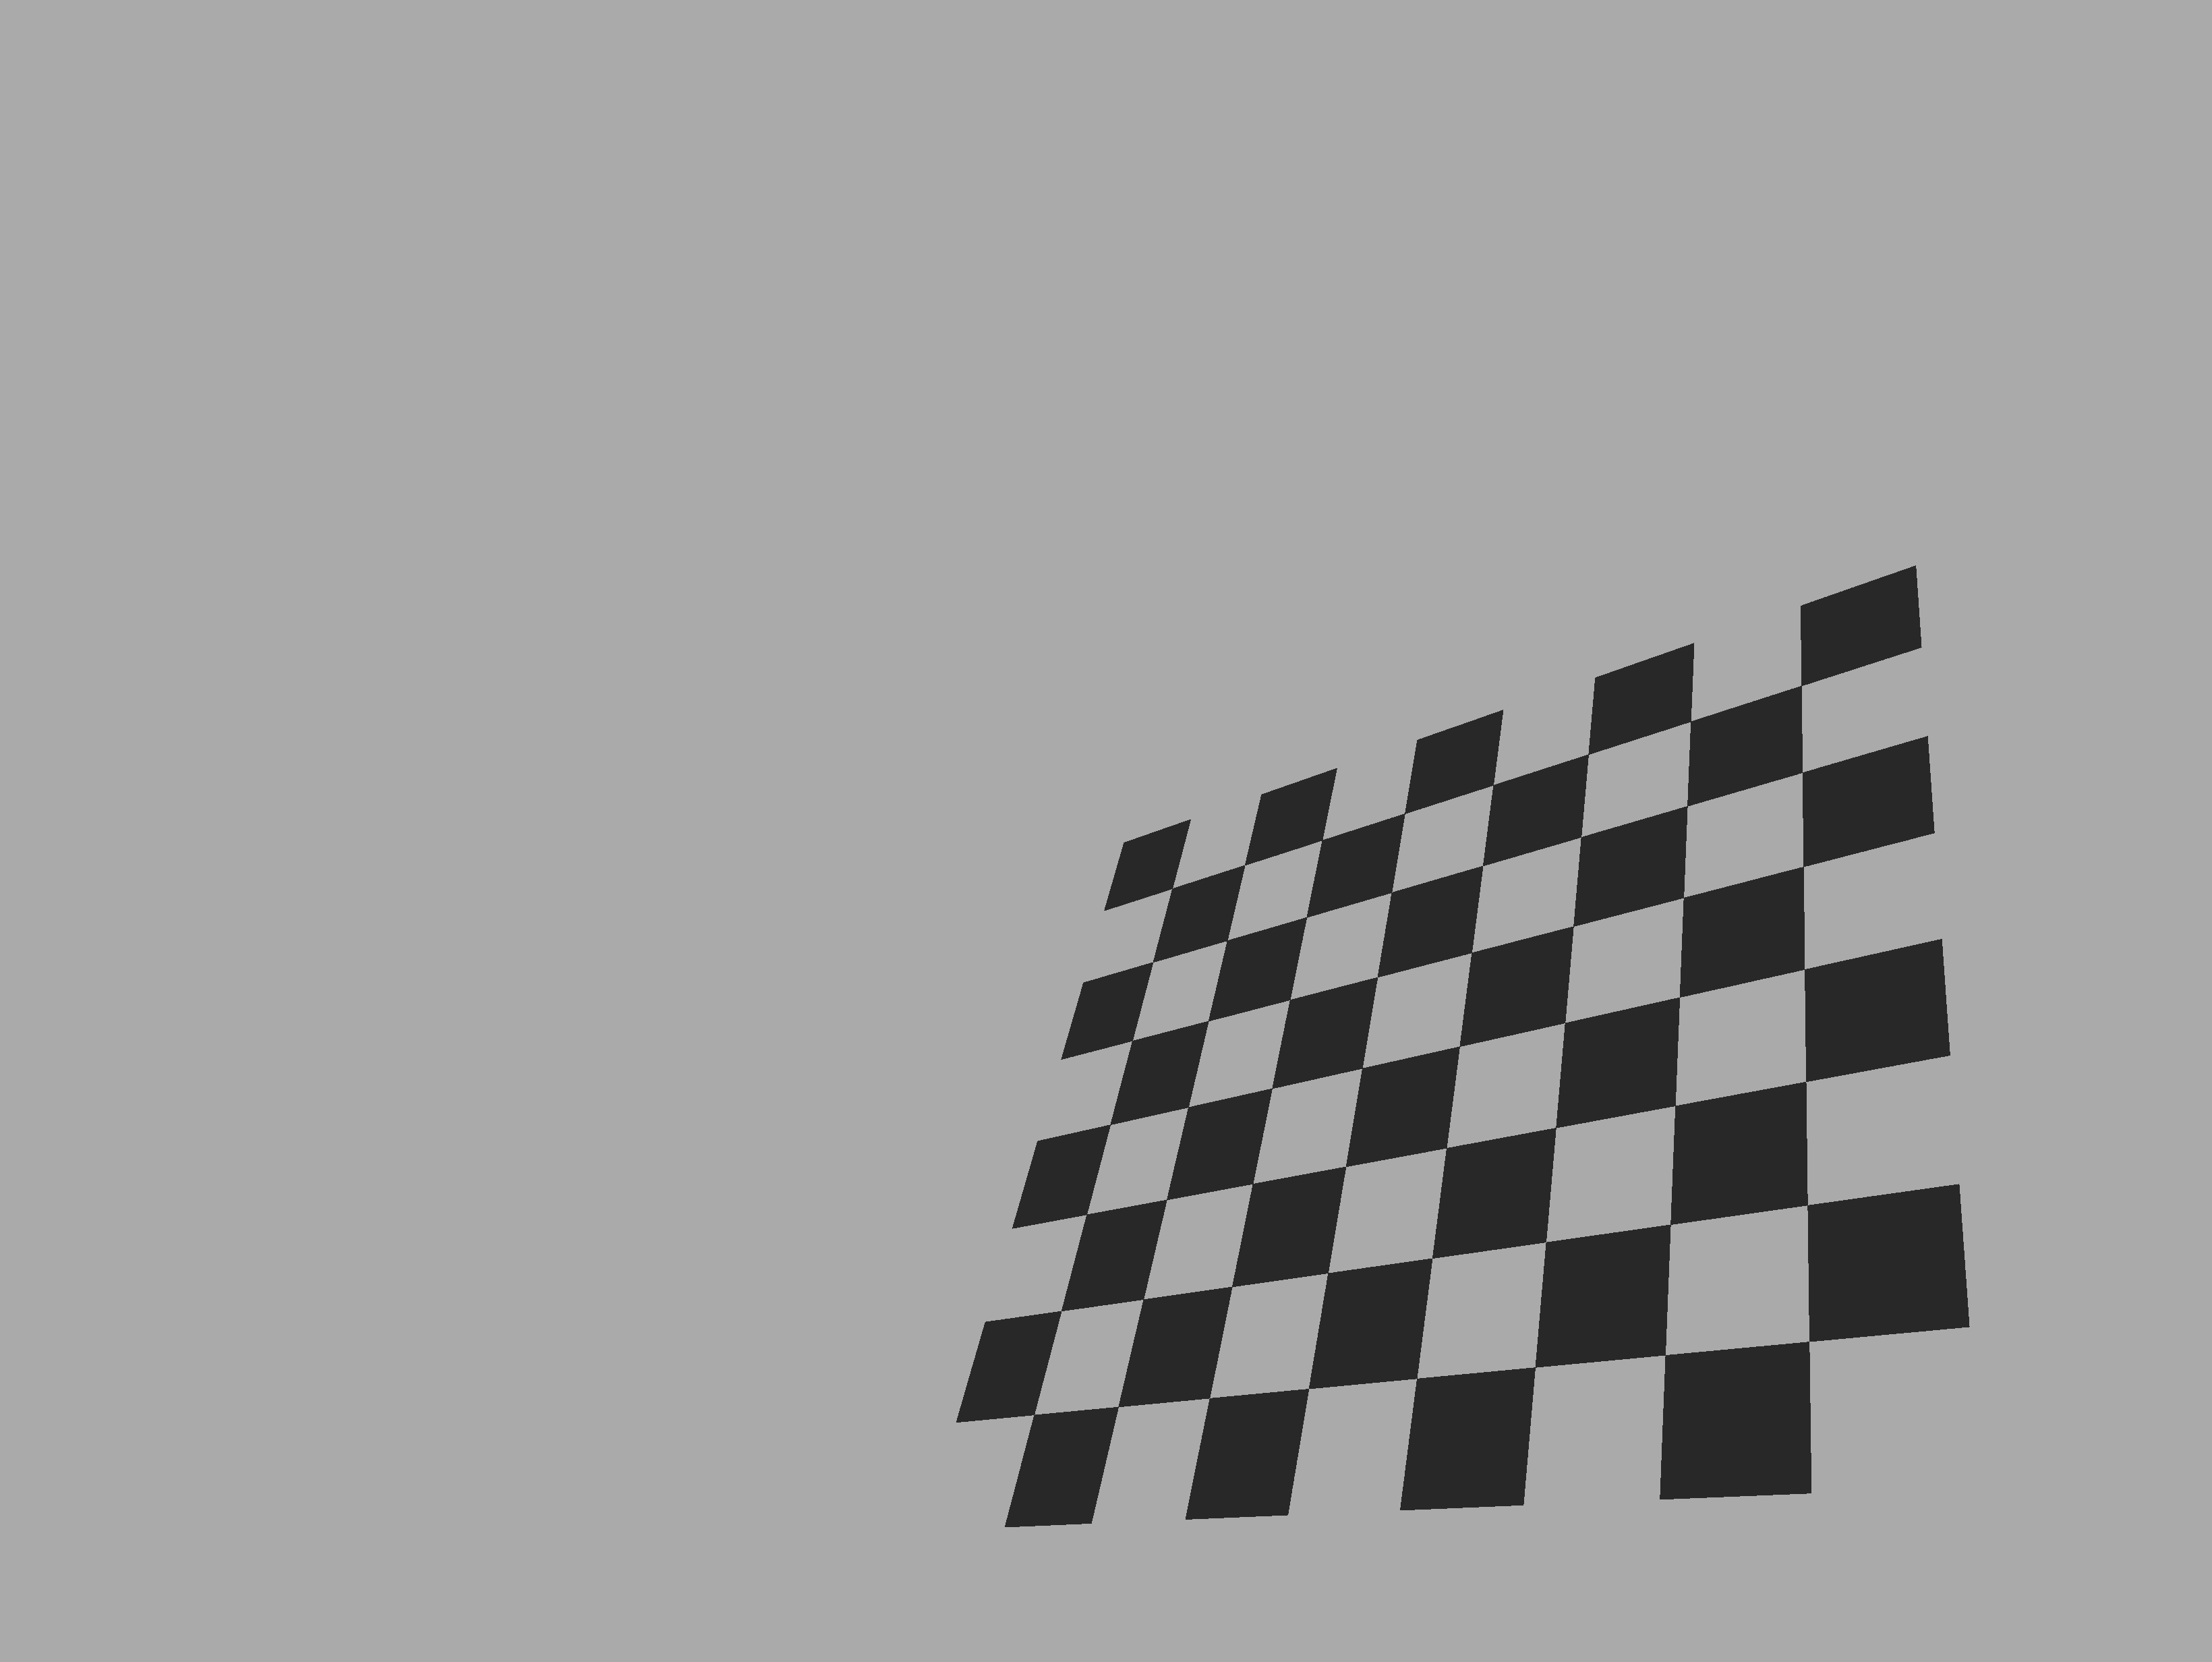
\includegraphics[width=0.5\linewidth, height=5cm]{3-development/threshold/im1.png}}}
	\subfigure[\label{development:thre4}]{\fbox{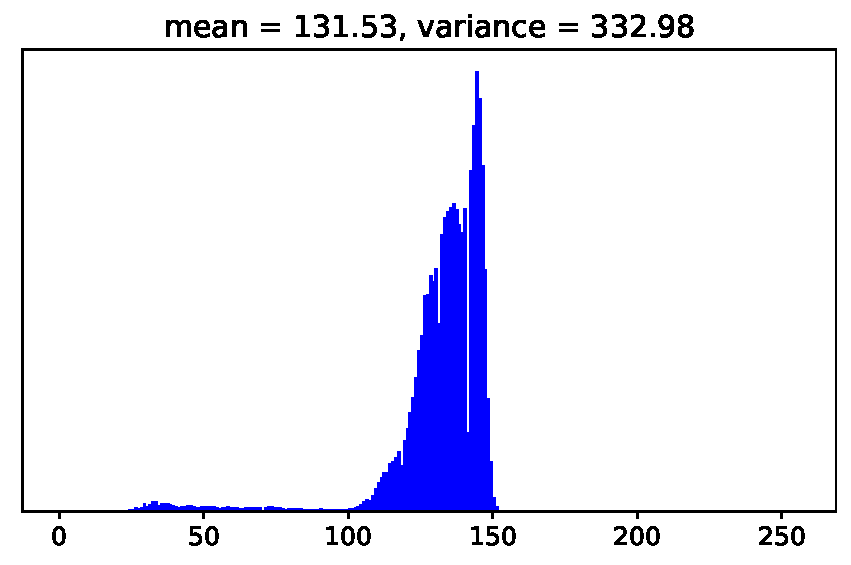
\includegraphics[width=0.5\linewidth, height=5cm]{3-development/threshold/hist_feder2.pdf}}}
	\caption{Histogram of the reference pattern and a spring with running back light\label{development:thre}}	
\end{figure}
In the picture \ref{development:thre1} the back light is running and the calibration pattern is in place but no object to measure. The corresponding histogram \ref{development:thre2} shows that nearly every pixel belongs to the background white which is between the value 100 and 155. If a object enters the field of view of the camera it is displayed as black and we get more smaller values. This shift is also reproduced by the variance. The mean itself is getting corrected by the ISP and can not be used to detect if an object is in the image or not.\\


The obvious answer for a threshold would now be to just cut the histogram around the value 100 in two and set the values to black and white. But with the automatic ISP there is a good chance to loose important information if there is no adaptive threshold. Since the goal is to get as much information as possible from the edges, a little bit of noise can be handled. The method which produced the best results with a back light, was the triangle method. 
\begin{figure}
	\centering
	\fbox{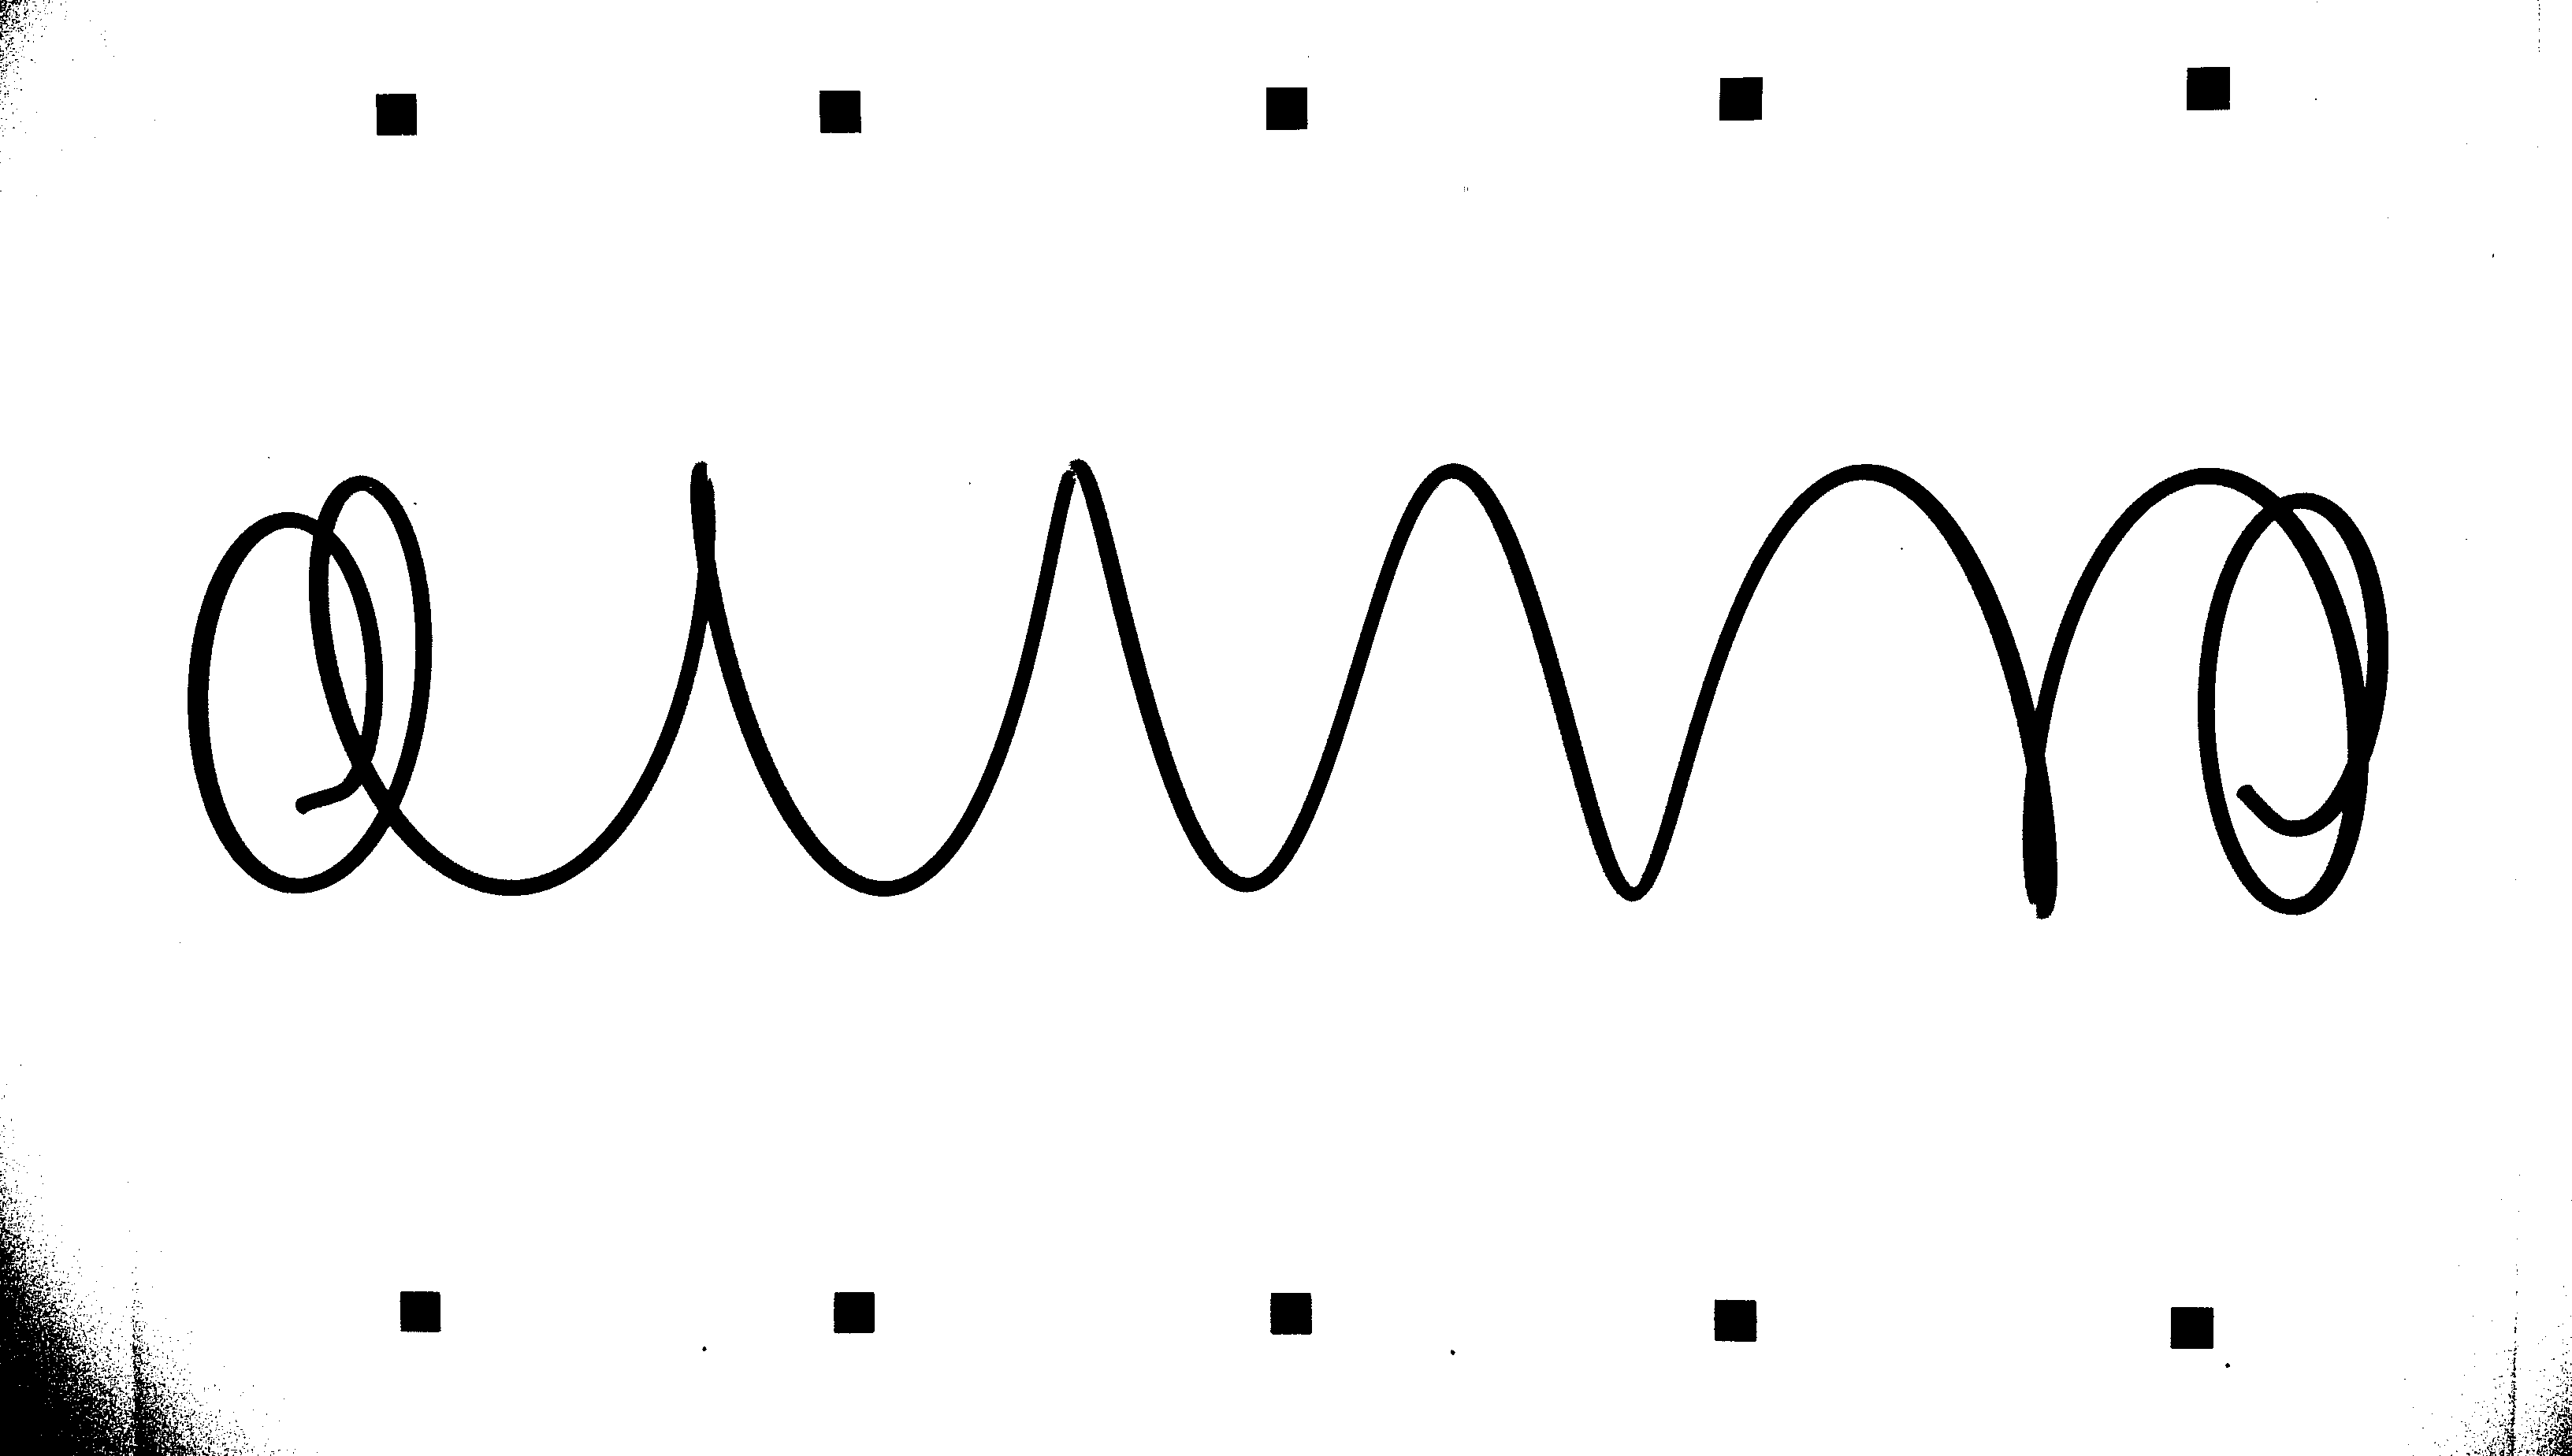
\includegraphics[width=\linewidth]{3-development/threshold/threshold.png}}
	\caption{Image after triangle threshold}
	\label{development:thresh}
\end{figure}
\begin{figure}[ht]
	\subfigure[\label{development:thre1}]{\fbox{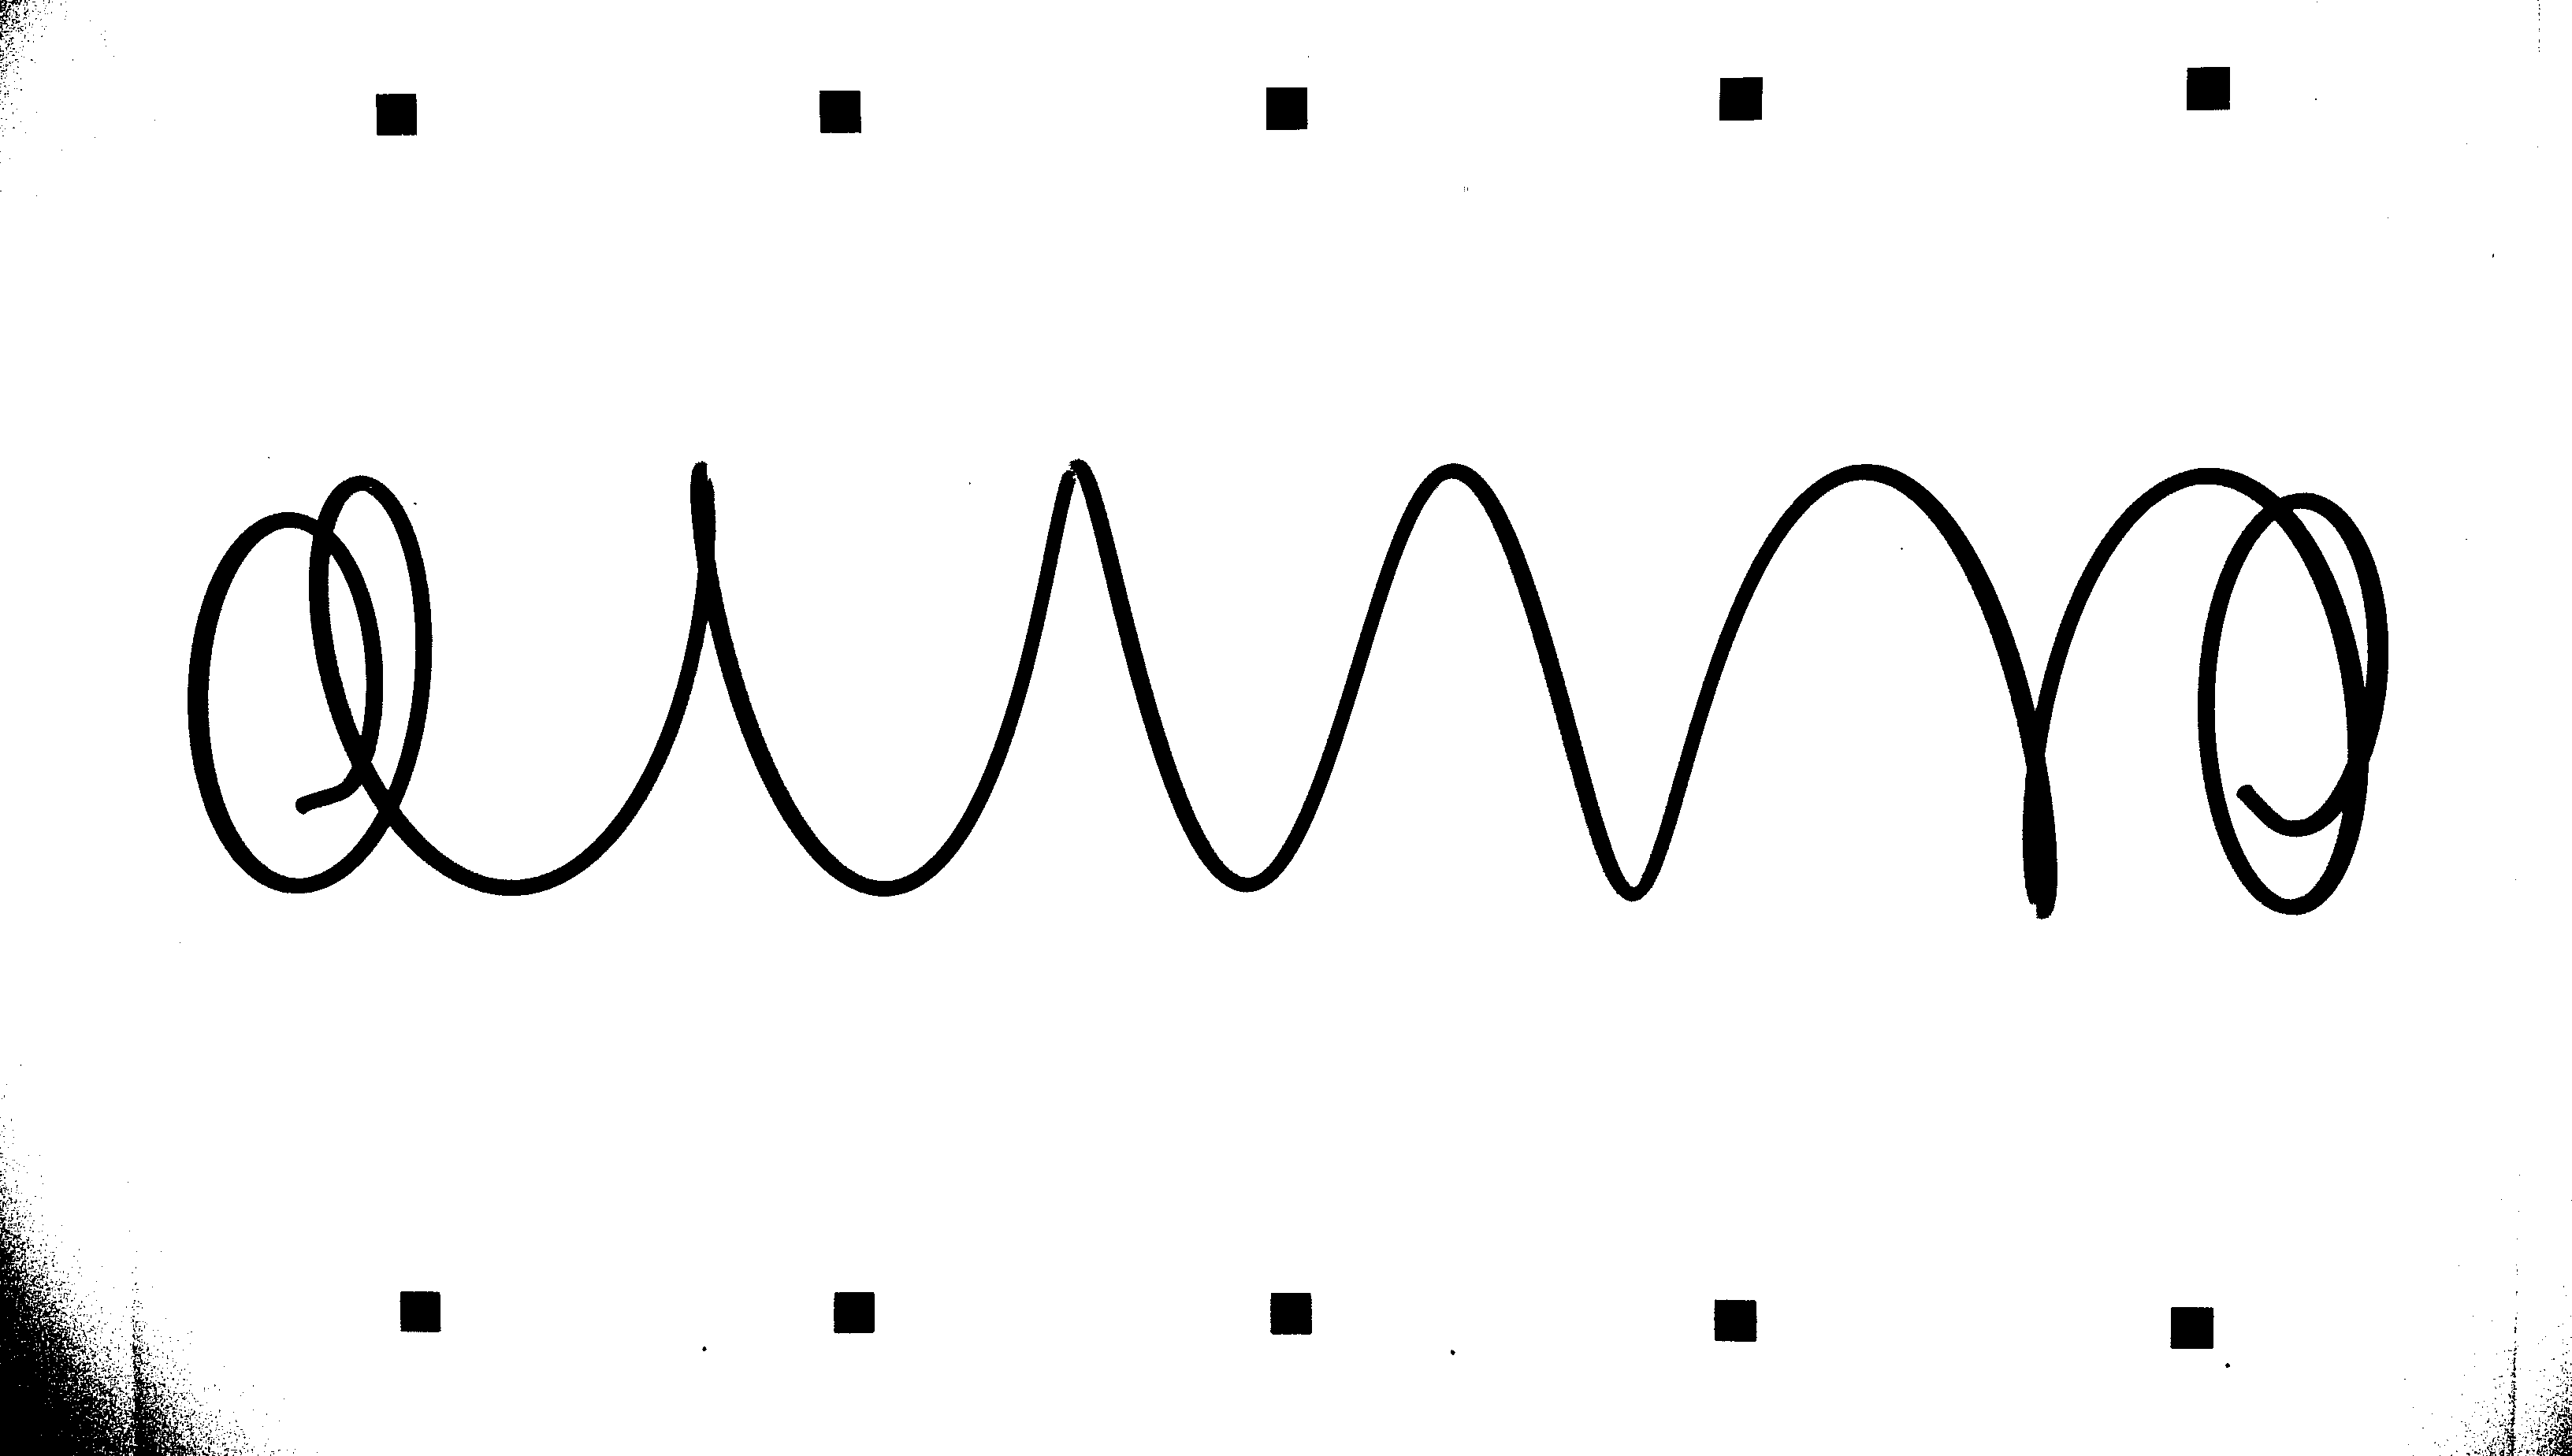
\includegraphics[width=0.5\linewidth, height=5cm]{3-development/threshold/threshold.png}}}
	\subfigure[\label{development:thre2}]{\fbox{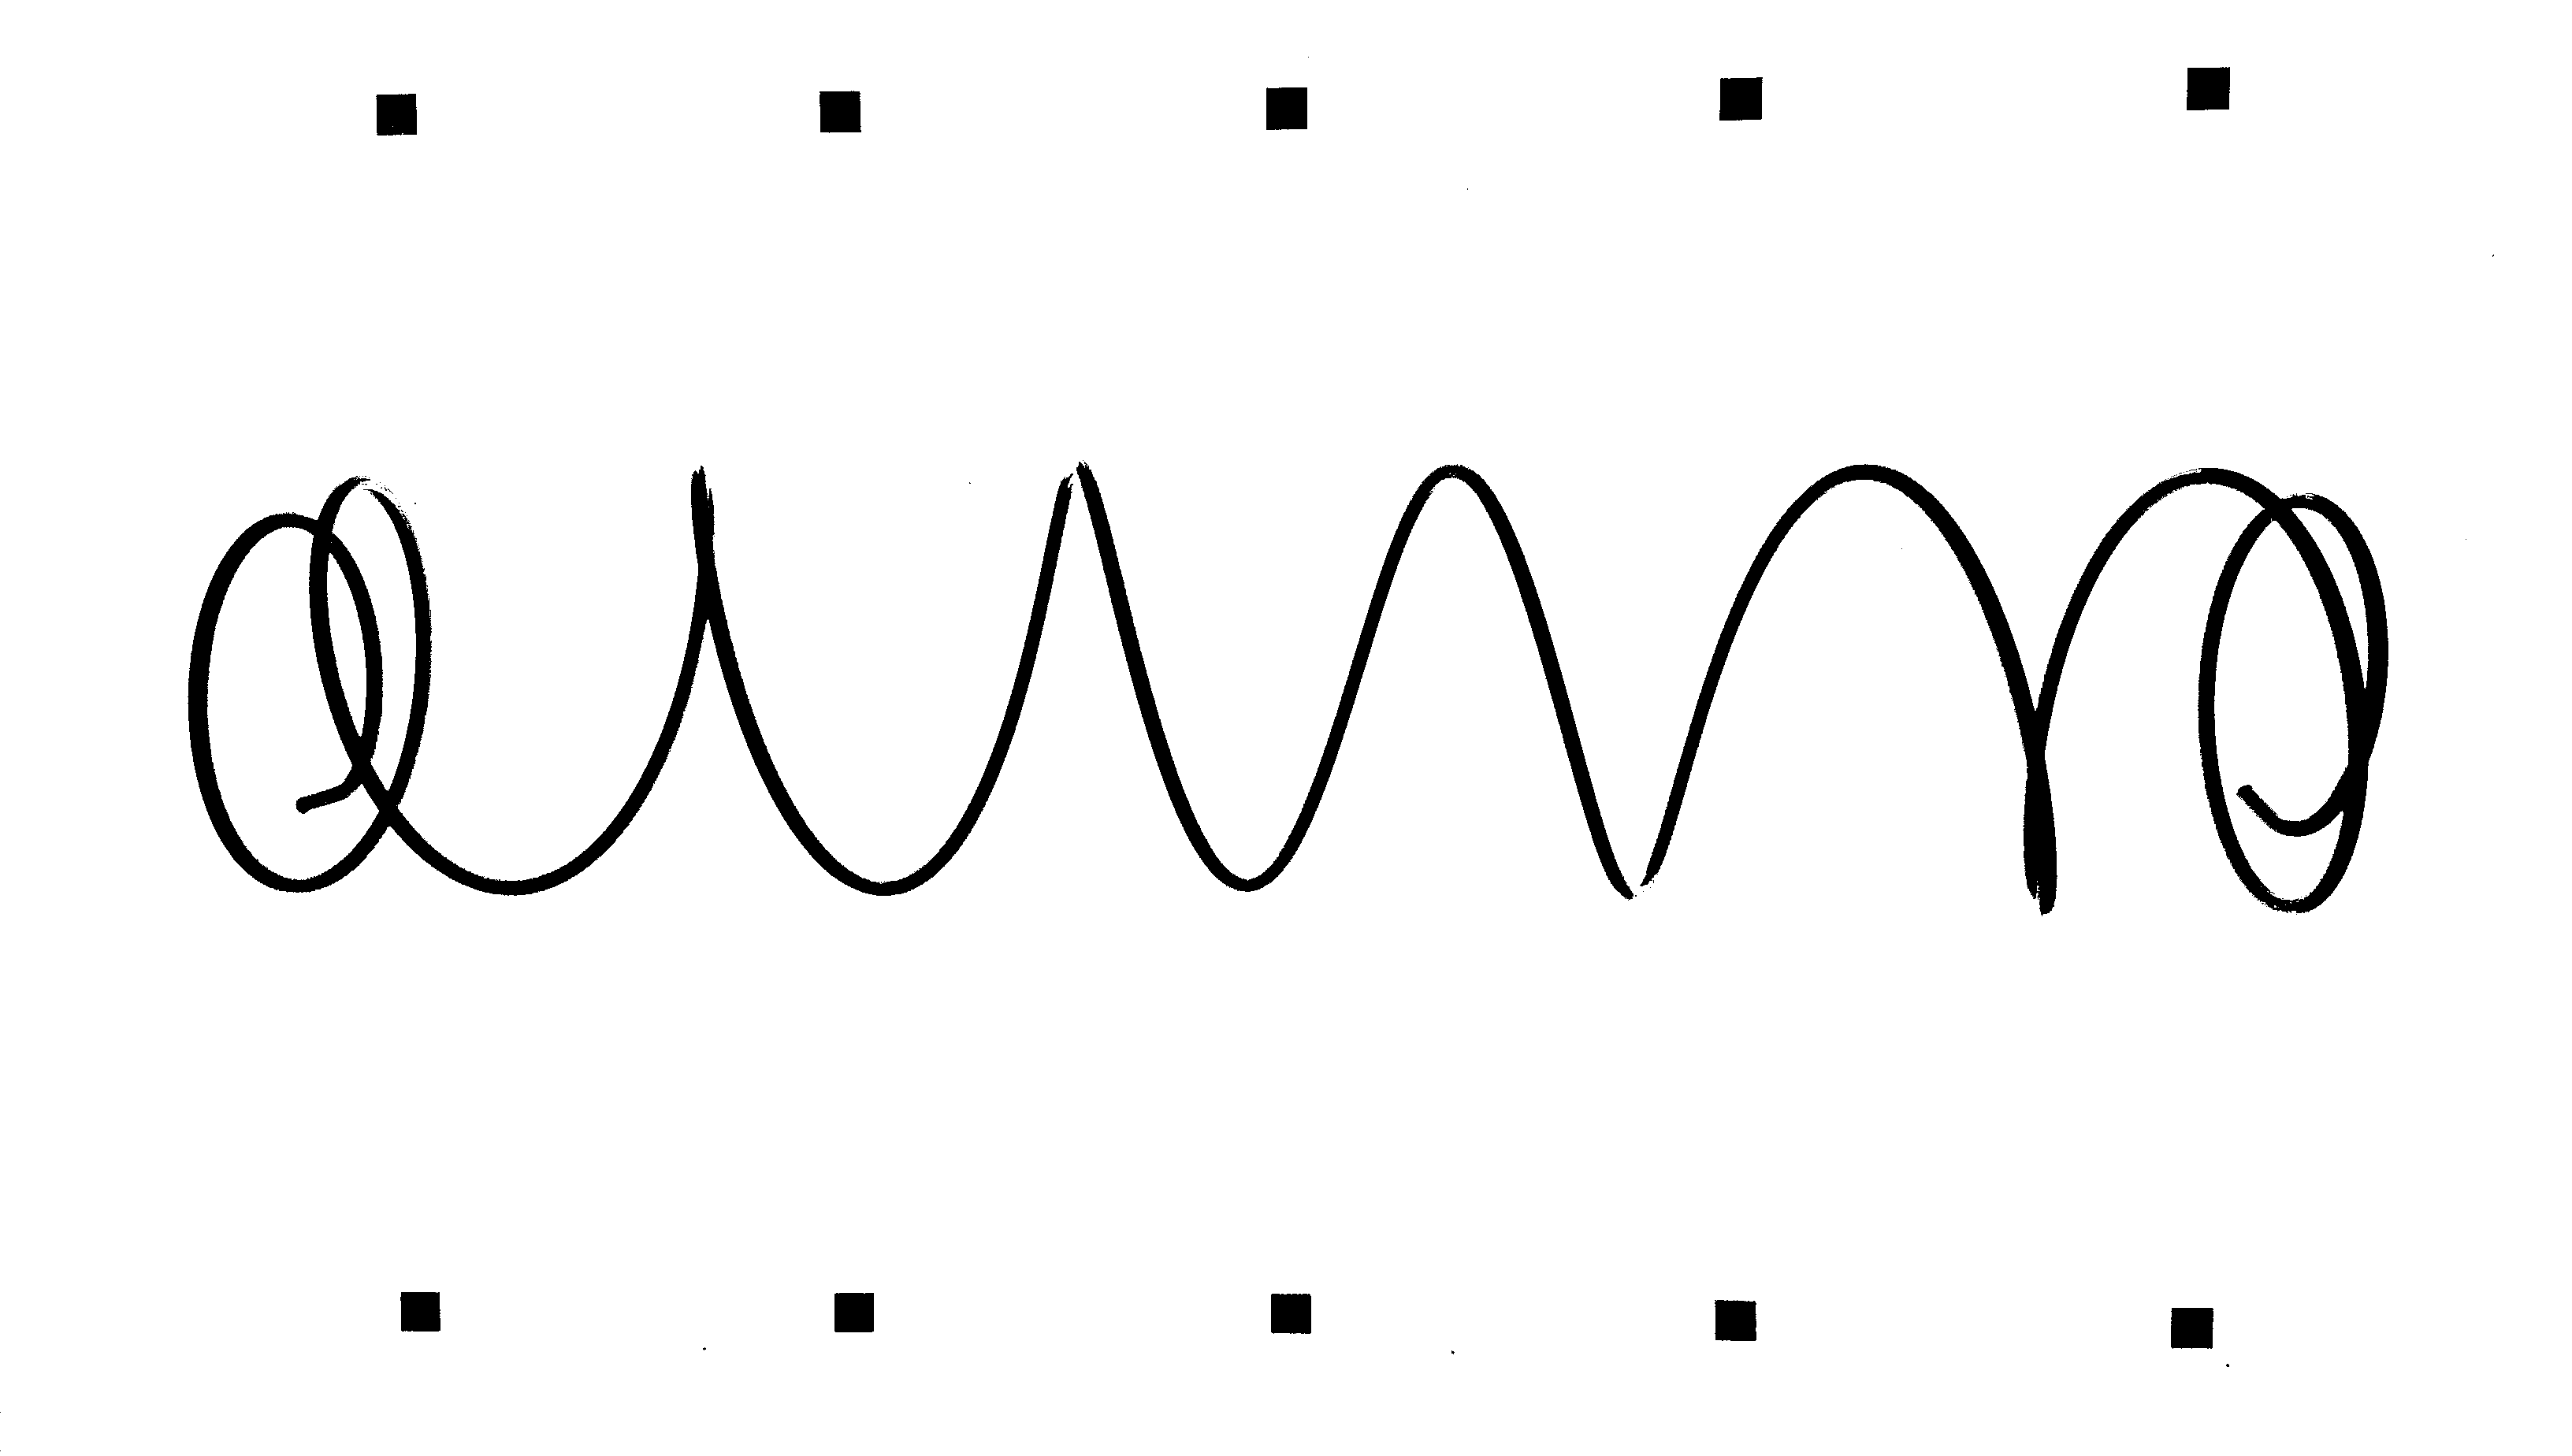
\includegraphics[width=0.5\linewidth, height=5cm]{3-development/threshold/otsu.png}}}
	\subfigure[\label{development:thre3}]{\fbox{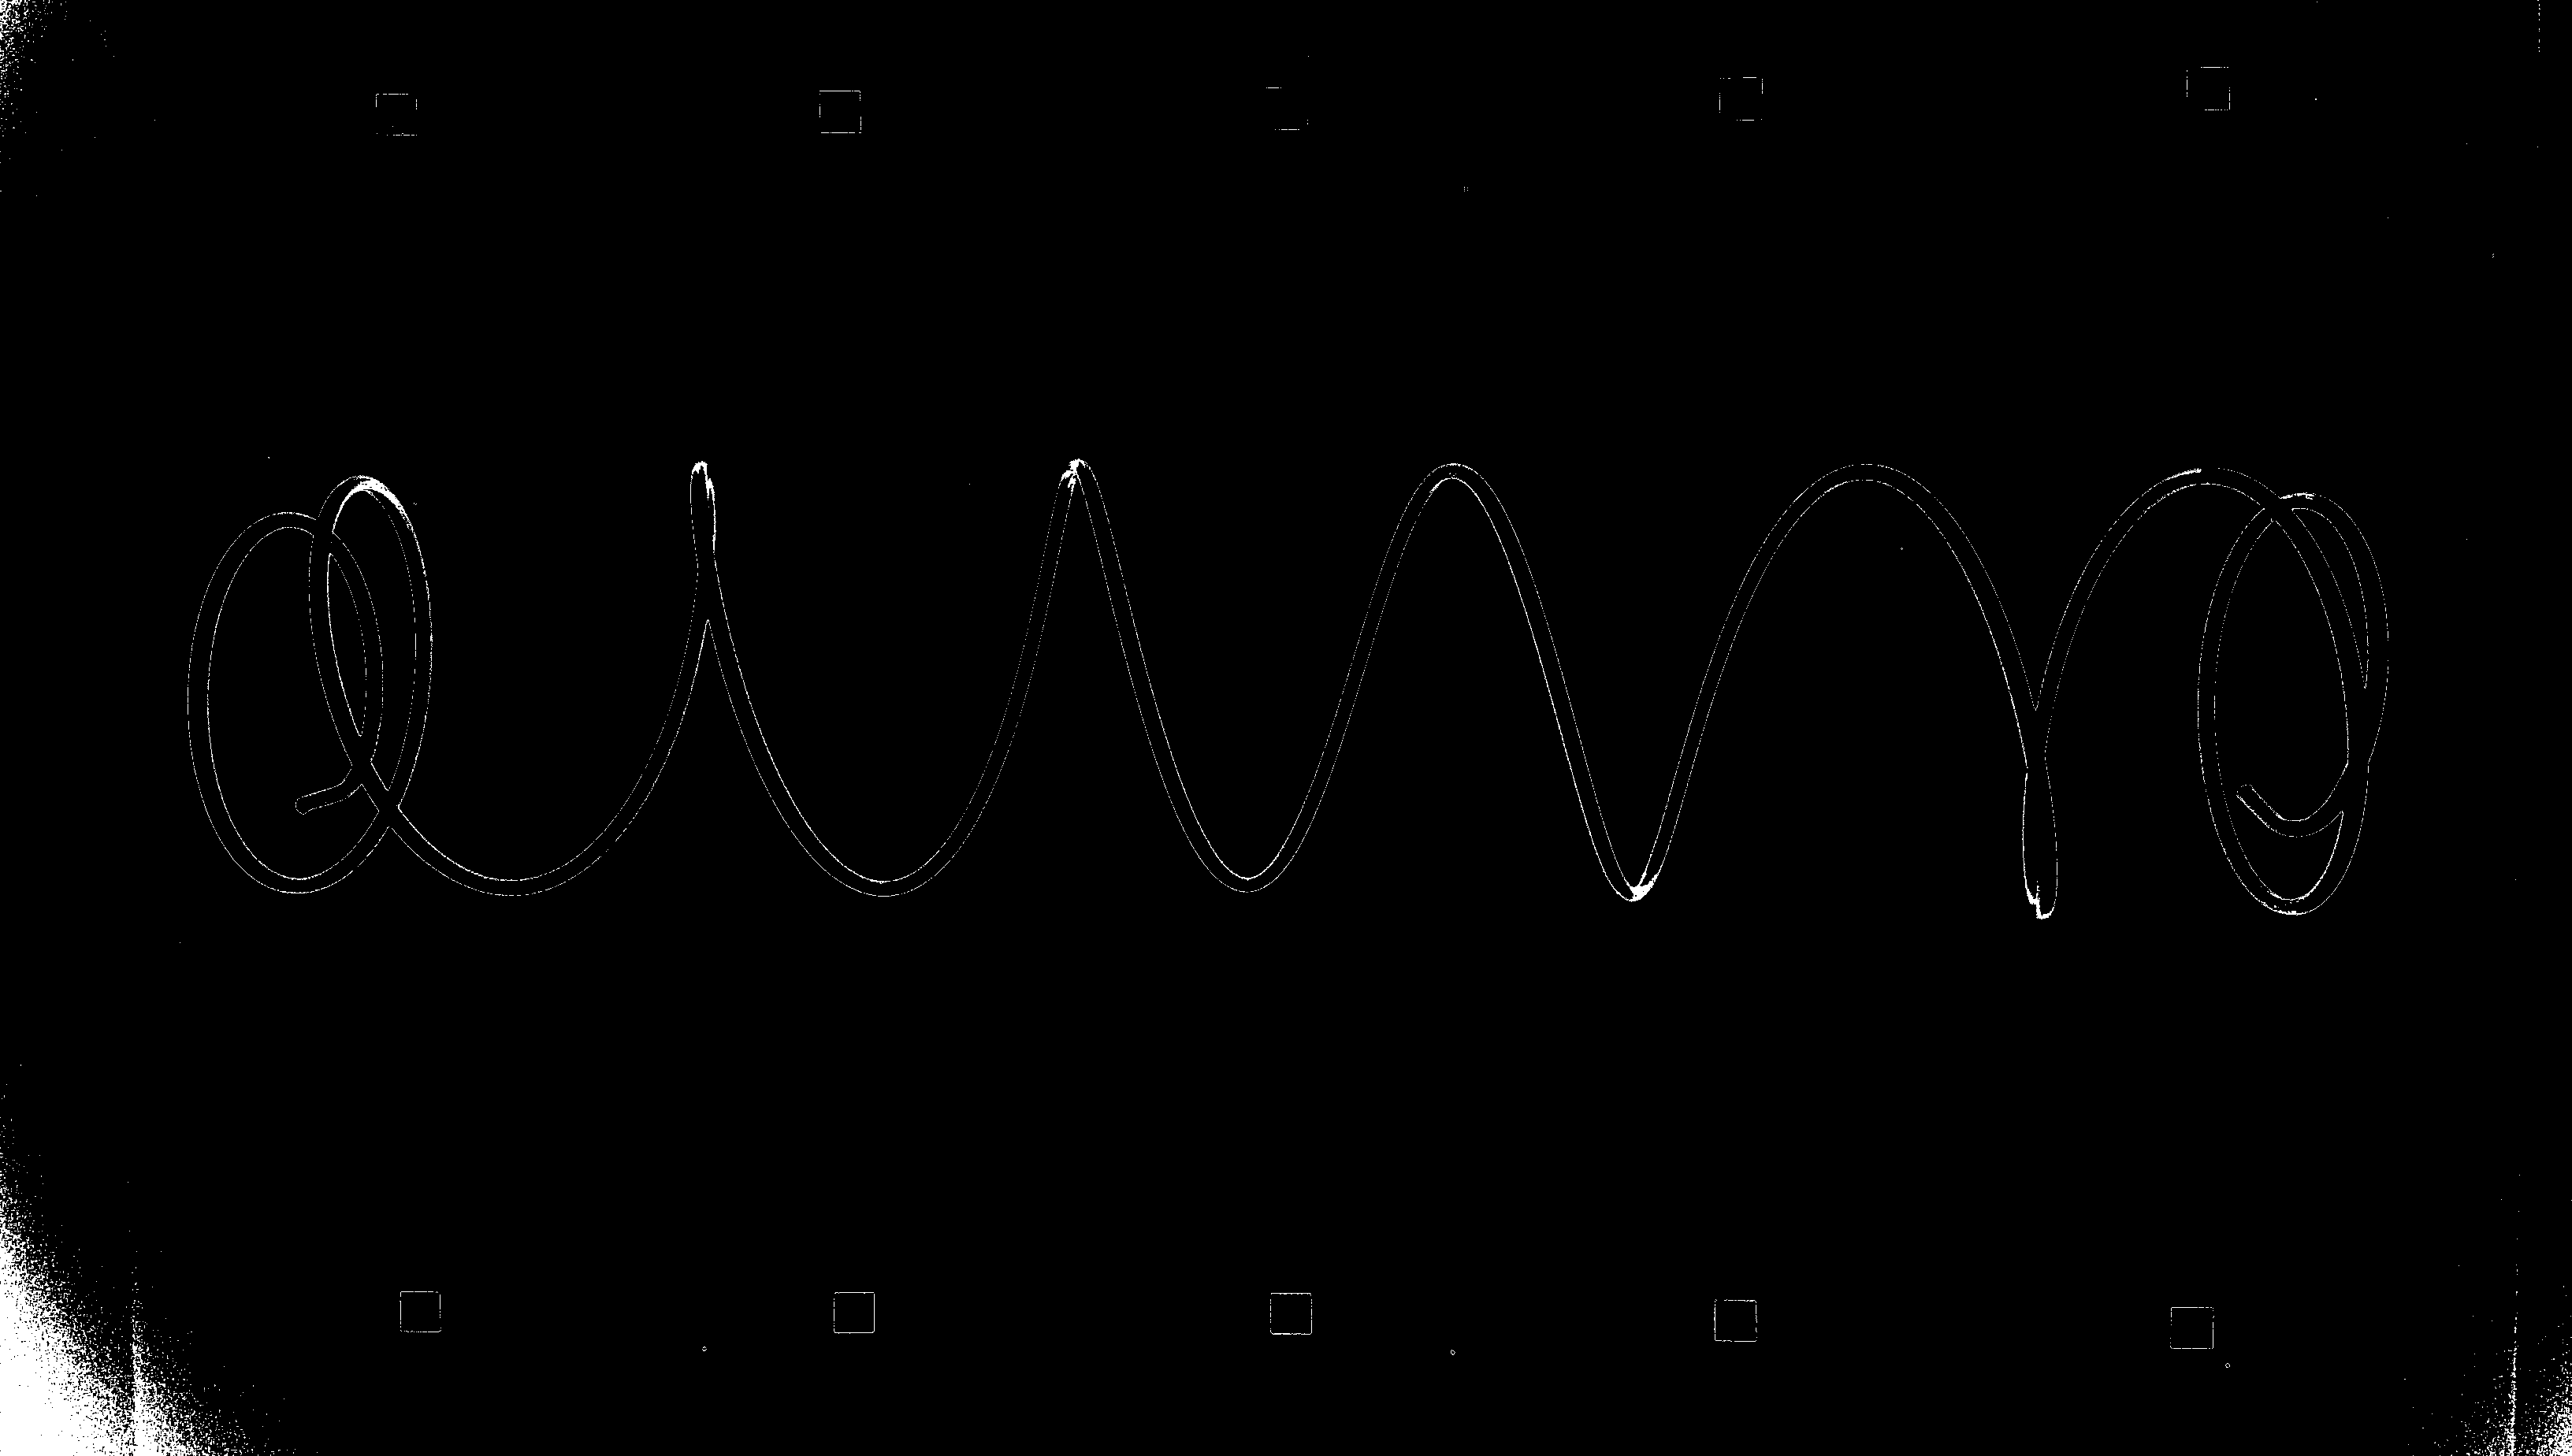
\includegraphics[width=1\linewidth]{3-development/threshold/diff.png}}}
	\caption{Comparison between otsu and triangle threshold\label{development:diff}}	
\end{figure}


\begin{figure}
	\centering
	\fbox{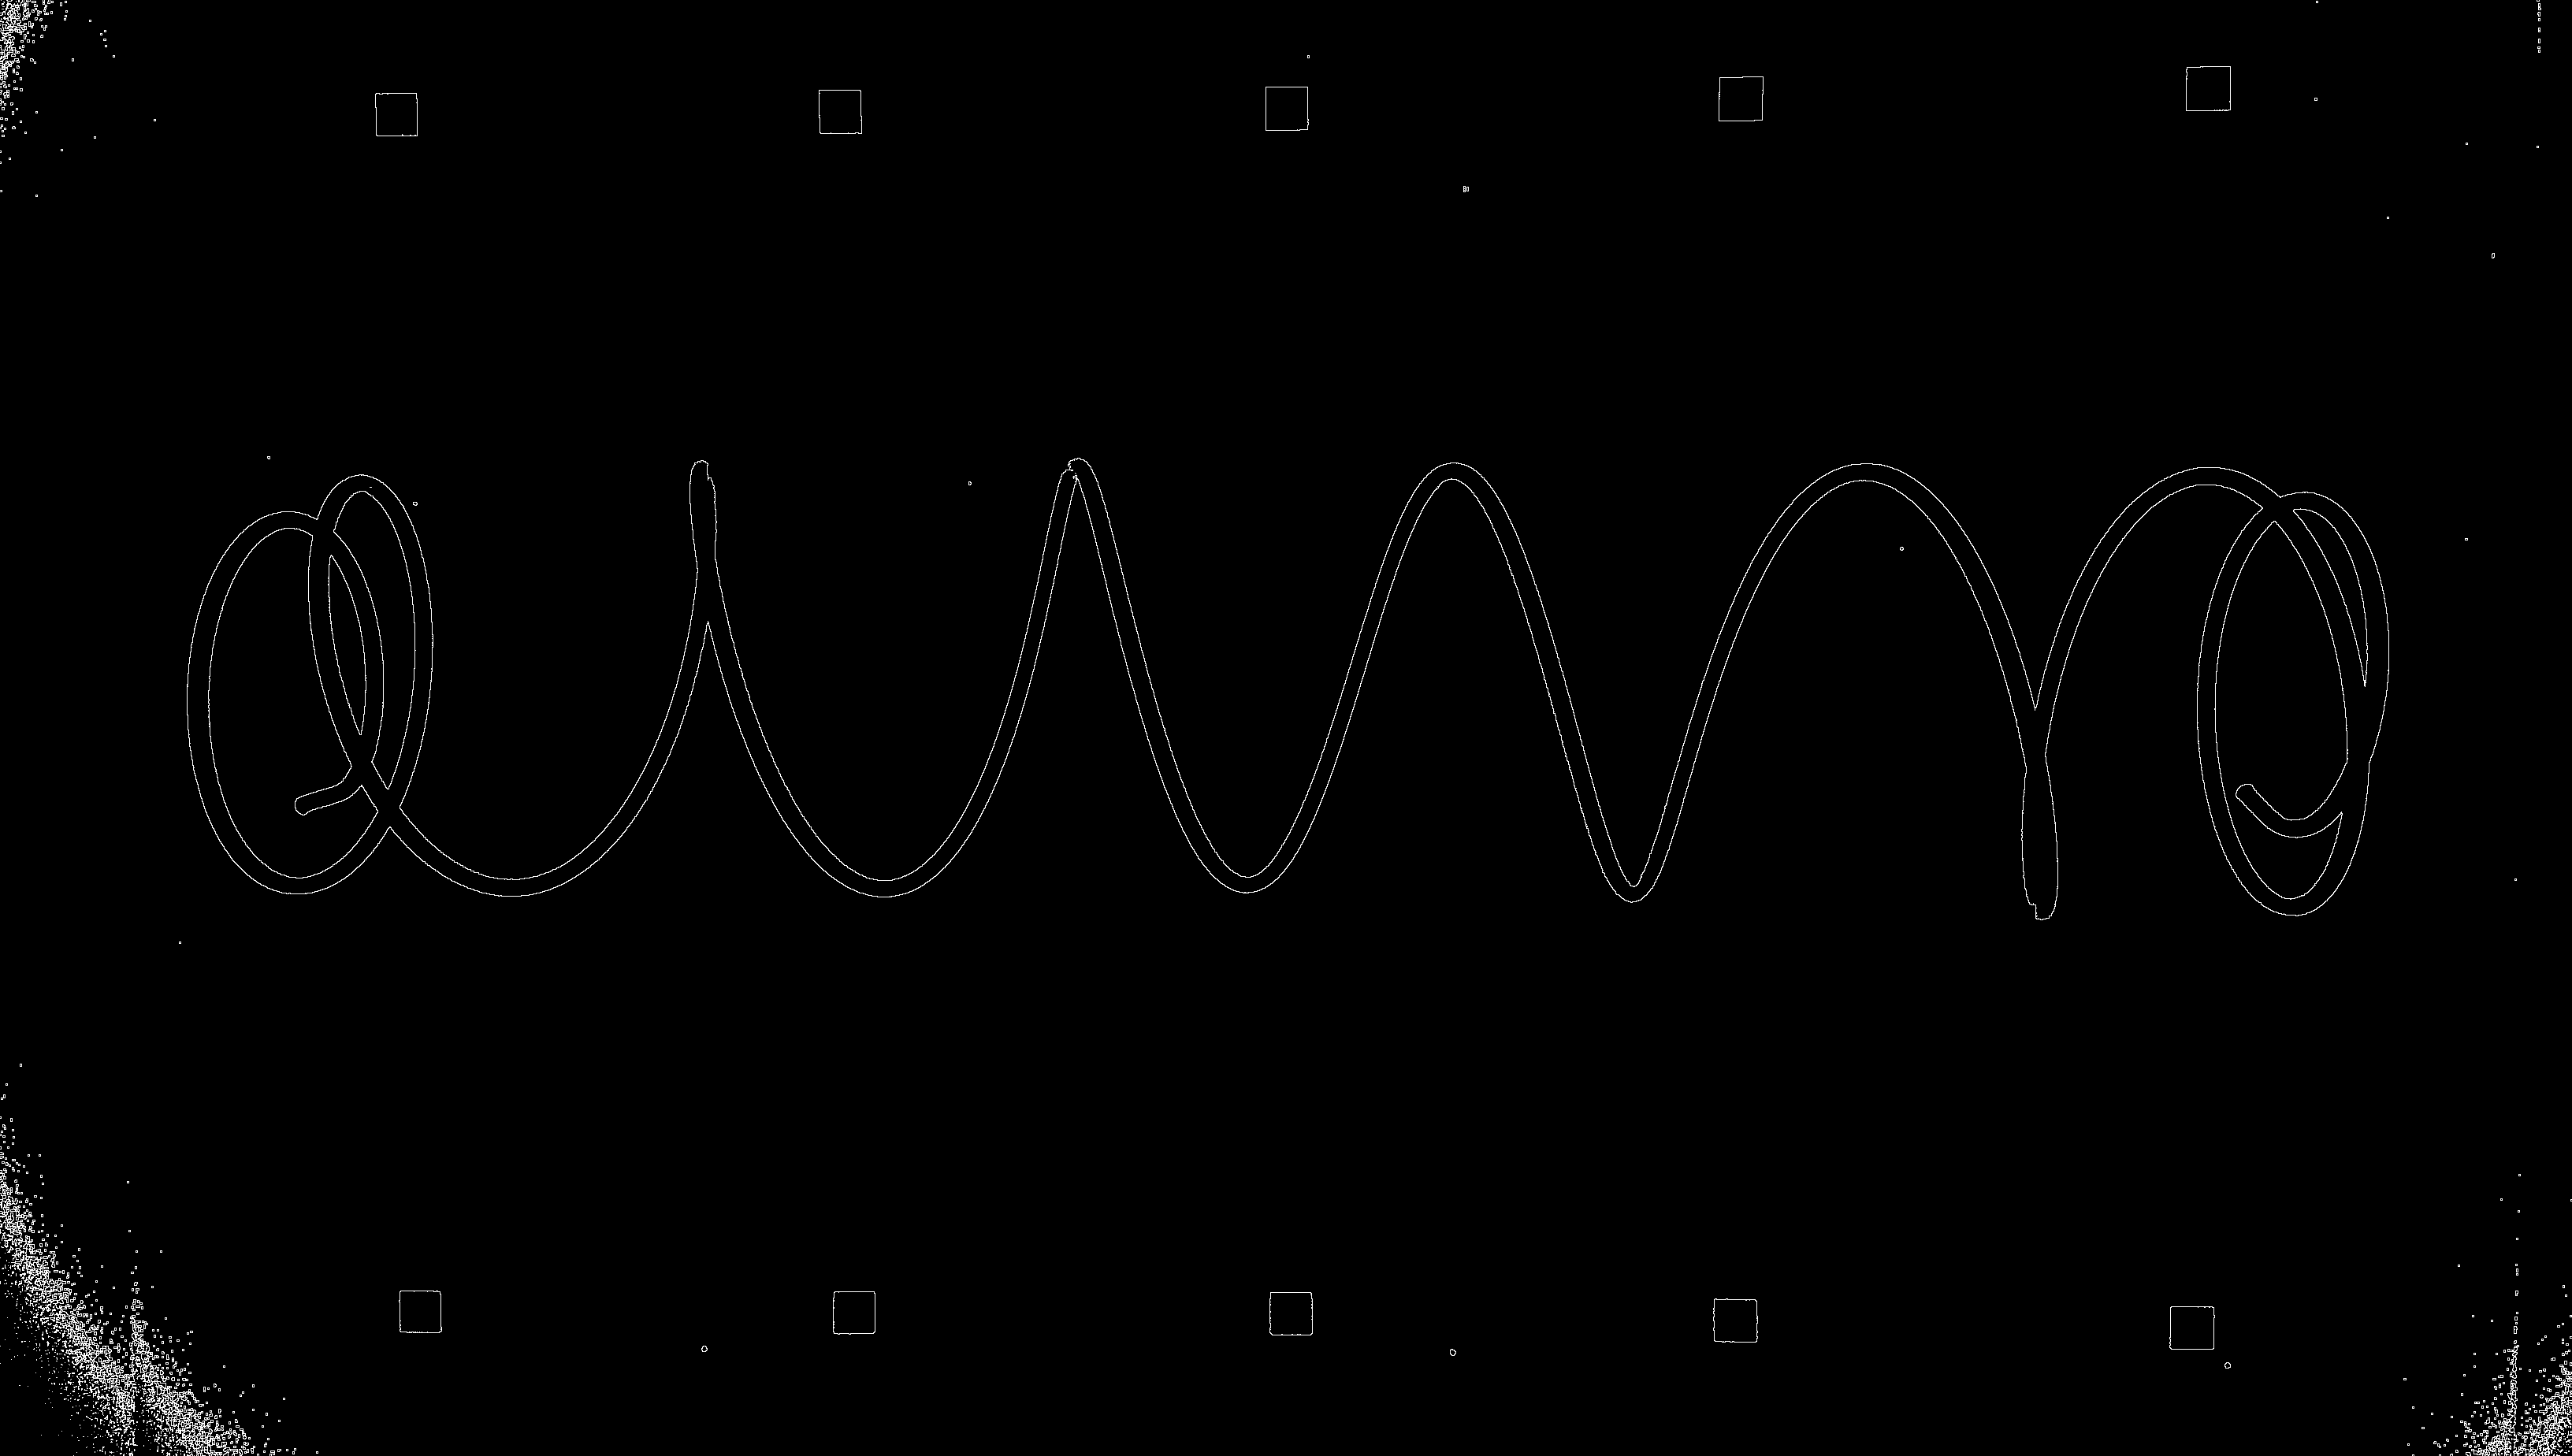
\includegraphics[width=\linewidth]{3-development/threshold/edge.png}}
	\caption{Edges of given image with morphological detection}
	\label{development:edge}
\end{figure}
